	\section {Virtual Machine Taxonomy Proposal} \label{sec:taxonomiaPropuesta}
	
	\begin{figure*}[ht]
		\centering
		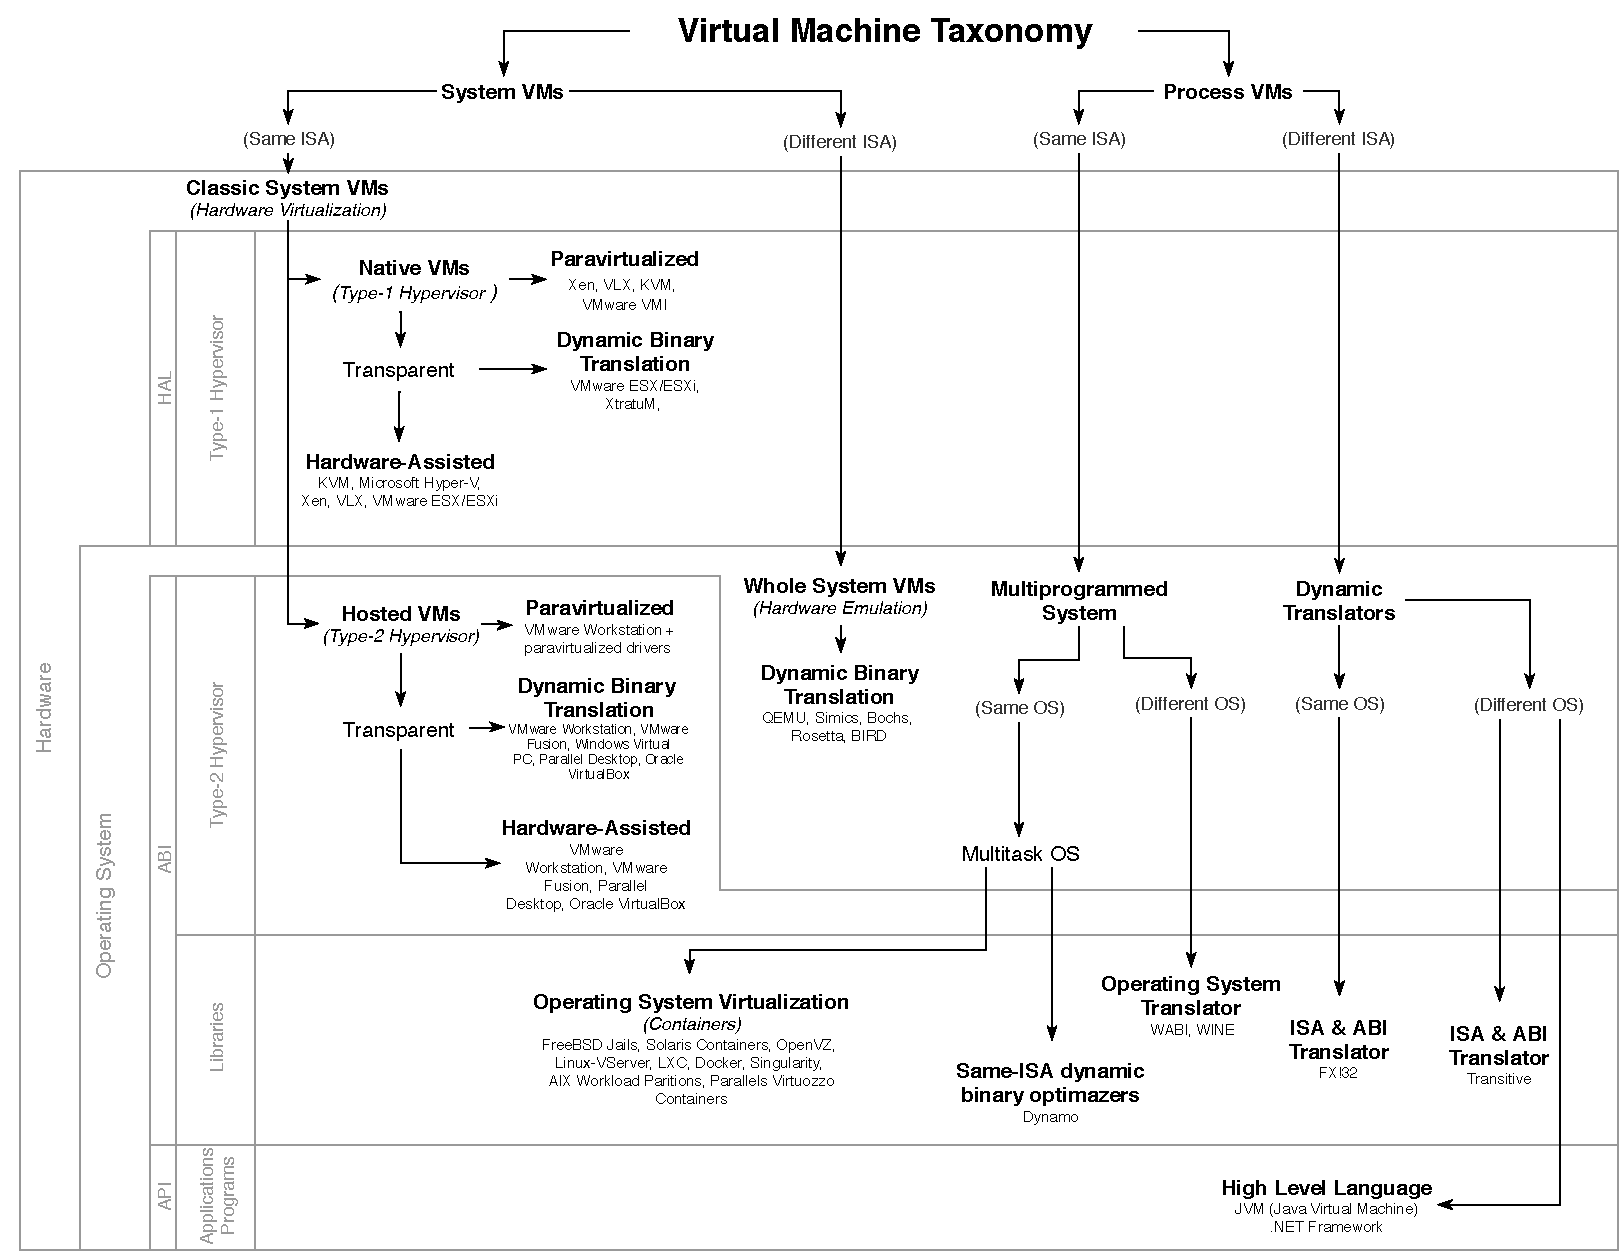
\includegraphics[width=17cm]{images/virtualMachineTaxonomy.pdf}
		\vspace{-0.2cm}%
		\caption{Virtual Machine Taxonomy Proposal. This taxonomy shows the outdated names of virtualization technologies that have lost validity. However, these names are still used to help the community to understand the positions within this new taxonomy. It is also important to include virtualization technologies that have gained full recognition in the industry and academia, such as \textit{Docker} and \textit{Singularity} among others. }
    	\label{fig:TaxonomiaPropuesta}
	\end{figure*}
	
	Starting from the concept of taxonomy as the science of naming things and classifying them into different groups \cite{CambridgeDictionary2018, Chi2000}, the taxonomic proposal technologies related to VMs is presented below. According to \textit{Chiueh} \cite{Chiueh2005} and \textit{Hoopes} \cite{Hoopes2009}, virtualization can occur either by aggregation (many elements are seen as one) or by a division of resources (one element looks like many). It is essential to clarify this point, as the taxonomy proposed in this paper focuses on aspects related to virtualization by \textit{resource division}. We also focus on server virtualization. We recommend that classifications of resource aggregation be kept separate from classifications of resource division. We note that studies like Kampert, Kusnetsky and Ameen which consider other types of virtualization do little to break down categories other than server/CPU virtualization. Thus we recommend that classifications of types of virtualization be kept separate from classifications of how server/CPU virtualization is implemented.  
	
	
	%JNM Say a bit more clearly why you are rejecting Kusnetsky and Kampert?  Mention Pessolani specifically too.. you are keeping that one also yes?
	
	%We chose not to include the taxonmies of Kusnetsky and Kampert because they are including virtualization of other kinds of resources like storage and networking. 
	%Also give the reader a heads up on that earlier in the paper.. when you introduce them 
	%say they are worth mentioning but beyond your scope in this paper or something like that
	
	%LESR new
	
Our proposed taxonomy, focused on resource division and server/CPU virtualization, builds based on the twelve reviewed studies, but is particularly focused on the studies such as that made by \textit{Chiueh} in 2005 \cite{Chiueh2005}, \textit{Smith and Nair} in 2005 \cite{Smith2005}, \textit{SCOPE Alliance Virtualization Group} in 2008 \cite{SCOPEAlliance2008}, \textit{P{\'e}k et al.} in 2013 \cite{Pek2013} and \textit{Bugnion et al.} in 2017 \cite{Bugnion2017}.
	
	Our taxonomy integrates the taxonomic approaches \textit{Level of abstraction} and \textit{Type of VM}. The first approach is oriented towards the use of layers, based on the levels of abstraction of the classical architecture of a computer system. The second approach is oriented towards the types of virtual machines that are either system or process. See Figure \ref{fig:TaxonomiaPropuesta}. 
	
	% Old
	%The \textit{Virtualization domains} approach was not considered in the present taxonomy.  This because some of the identified domains represent an interesting bet in the effort to organize elements or technological resources related to virtualization, but these are outside of the definition of virtualization made by \textit{Goldberg} \cite{Goldberg1973}, which is the approach followed in this paper. Therefore, in this taxonomic proposal, the integration of the \textit{Abstraction Level} and \textit{Virtual Machine Type} approach aims to present a way of visualizing the virtualization technologies related to VMs. This taxonomy allows the simultaneous display of the type of VM and its respective level of abstraction. The following sections, set out the taxonomy approaches contained in this proposal.
	
	%LESR new
	
	%The virtual machine taxonomy proposed here seeks to maintain consistency with the theoretical principles established in the definition of virtual machine given by Popek \cite{Popek1974} and Goldbert \cite{Popek1974, Popek1974}. In this sense, the domains "Type of VM" and "Level of abstraction" fit properly, however, the Domains of virtualization approach does not do it completely. This is why some categories of work using this approach will not be taken into account for inclusion in this proposal. For example, the security and administration and desktop domains described in Kampert's work; the access and administration categories of Kusnetzky's study and the Resource, grid and cloud virtualization categories of Abdulhamid's work, among others. 
	
	
	
	\subsection{Taxonomic Dimension 1: Abstraction level}

	This approach is based on the use of labels to determine layers similar to the levels of abstraction of a computer system, such as: Hardware, HAL, Operating System, ABI, API, Type-1 hypervisor, Type-2 hypervisor.   In Figure \ref{fig:TaxonomiaPropuesta}, the labels correspond to the levels of abstraction that are located on the left side. They also form the title of the rectangular structures with the horizontal distribution of the taxonomy. These rectangular structures identify a layer for the technologies contained in them.
	
	With the use of these layers, the taxonomy makes it possible to locate virtualization technologies depending on the level at which they take place. Thus, the reader can quickly infer aspects such as the dependence or not of an underlying OS and also determine the number of intermediaries involved in the virtualization process. This therefore allows us to infer in some occasions, the possible performance of these technologies.
	
	With regards to the HAL layer, the presence of a Type-1 hypervisor category can be seen. It also makes hardware-assisted virtualization technology visible in architectures such as x86. Both labels show that this type of hypervisor is directly placed over the hardware.  This arrangement is called \textit{bare-metal} and it is identified by the absence of intermediaries between the VMs and the hardware, which suggests a higher performance for the set of technologies located in this layer.
	
	The layer corresponding to the OS shows other technologies that apply virtualization through the presence of independent Type-2 hypervisors, or in conjunction with the technologies that assist virtualization from the hardware. This layer also indicates that virtualization is carried out through ABI using calls to the OS and using the latter as an intermediary between host systems and hardware. This situation suggests that the virtualization technologies belonging to this layer may present an inherent degradation in performance due to the costs of intermediation between the different environments.
	
	In the same layer, its also shows that there are virtualization technologies based on segmenting the OS in light operational environments, currently known as containers. To a large extent, they can contrast performance degradation because they do not perform virtualization of a complete OS.
	
	The last level of abstraction shows virtualization technologies that use APIs as a base. In the case of high-level languages, these can offer a high level of portability because generally, the APIs are used for multiple hardware and software platforms.
	
	\subsection{Taxonomic Dimension 2: Type of VM}
	
	First, VMs are considered as \textit{System VMs} or \textit{ Processes VMs}. 
	
	%In Figure \ref{fig:TaxonomiaPropuesta}, this approach corresponds to the interpretation of \textit{top-down}.
	
 \textit{System VMs} contain within their virtual environment a complete OS (guest OS) while \textit{Process VMs} do not. Instead, Process VMs use the \textit{host} OS as an intermediary between the virtual environment and the real hardware. A description of each category follows.
 
 Notice that some specific products appear in more than one category when they offer different modes of operation.
	
	\subsection{System VMs}
	
	The \textit{System VMs} are divided into two categories.  The first category is called \textit{Classic System VMs} where both host and guest use the same ISA. The second category is called \textit{whole system virtual machines} where the host and guest use different ISA.
	
	\subsubsection{Classic system VMs} This type of virtualization is also known as \textit{Hardware Virtualization}, and in turn includes two categories, the first one is called \textit{Native VMs} and the second one \textit{Hosted VMs}. It is important to note that each of these categories takes place at different levels of abstraction.
	
	\textbf{Native VMs}: This category is also known as \textit{Type-1 Hypervisors} and corresponds to the HAL abstraction level. Its characteristic is using a software layer directly on top of the hardware. It also presents a subdivision as shown below:
		
	\begin{list}{$\bullet$}{\setlength{\leftmargin}{5pt}}

			\item \textbf {Transparent} refers to VMs whose guest OS is not aware of their virtualization status and can finally be classified as \textit{Hardware-assisted} or \textit{dynamic Binary Translation}.
			
			\begin{list}{$\diamond$}{\setlength{\leftmargin}{8pt}}

				\item \textbf{Hardware-Assisted} virtualization involves the use of physical components to facilitate the management of virtual machines. This category includes examples such as KVM, Microsoft Hyper-V \cite{Kappel2009}, Xen, VLX and VMware ESX/ESXi \cite{VMware2018Website}.
				
				\item \textbf{Dynamic binary translation} implies that the Type-1 Hypervisor catches and inspects the code of each guest OS request to convert it into a proper request towards the underlying hardware. For examples VMware ESX/ESXi and XtratuM \cite{XtratuM}.
				 
			\end{list}
			
			\item \textbf{Paravirtualized} is also known as \textit{operating system-assisted virtualization} \cite{VMware2008}, \cite{VMware2018Website} and refers to efficient communication between the guest OS and the hypervisor. This implies modifying the guest OS to be aware of virtualization and to take advantage of that condition. This category includes examples, such as; Xen, VLX, KVM and VMware VMI \cite{VMware2018Website}.
			
		\end{list}	
	

	

\textbf{Hosted VMs} also known as \textit{Type-2 Hypervisors}, correspond to the ABI abstraction level. The main characteristic of this type of virtualization is using a layer of software on a pre-existing OS. Furthermore, it also presents a subdivision as shown below:
		
	\begin{list}{$\bullet$}{\setlength{\leftmargin}{5pt}}
		
			\item \textbf{Transparent} refers to VMs whose guest OS is not aware of their virtualization status. These virtual machines are classified in \textit{Hardware-Assisted} or \textit{Dynamic Binary Translation}.
			
			\begin{list}{$\diamond$}{\setlength{\leftmargin}{8pt}}

				\item \textbf {Hardware-Assisted} involves the use of physical components to facilitate the management of virtual machines. This category includes examples, such as VMware Workstation, VMware Fusion, Microsoft Virtual PC, Parallel Desktop, and Oracle VirtualBox.
				
				\item \textbf{Dynamic Binary Translation} implies that the Type-2 Hypervisor catches and inspects the code of each of the guest OS's requests to convert it into a proper request towards the underlying hardware. Examples here include VMware Workstation, VMware Fusion, Microsoft Virtual PC, Parallel Desktop and Oracle VirtualBox.
				
%JNM - explain when a given example is listed under multiple categories.. review these.. are you sure they are all under both?


			\end{list}
			
			\item \textbf {Paravirtualized} refers to efficient communication between the guest OS and the Type-2 Hypervisor; which implies modifying the guest OS to be aware of virtualization and take advantage of that condition. An example of this category is VMware Workstation, with the addition of the corresponding paravirtualization \textit{driver} to the network in the guest OS \cite {VMware2018Website}.
			
		\end{list}	

	\subsubsection{Whole system VMs}
	This type of virtualization is also known as \textit{Hardware emulation} and takes place at the ISA abstraction level.  This emulation presents an ISA different from the underlying hardware. However, in the proposed taxonomy it is located at the ABI abstraction level, which makes evident the existence of a pre-existing OS on which emulation can occur.
	
	\subsection{Proccess VMs}
	
	The \textit{Process VMs}, as well as the \textit{System VMs}, present a division according to the ISA projected in the virtual environment. When the ISA is the same, the category is called \textit{multiprogrammed systems}; otherwise, the category is called \textit{Dynamic translators}. Both categories are initially located at the level of the OS. This indicates the dependence of a pre-existing OS with has the purpose of generating the virtual environment for the processes. Each of these categories and their respective derivations is described below.
	
	\subsubsection{Multiprogrammed systems}
	
	Multiprogrammed systems implement the ability to share the OS among many processes, generating independent execution spaces for each one. This generates the illusion that for a moment of time, a process is an exclusive executor in the system. This category is then divided into two depending on whether there is an OS. When the same OS is projecting, the category is called \textit{Multitasking OSs}; otherwise, they are called \textit{OS translators}.
	
	\textbf {Multitasking OS} is dividing in turn into \textit{OS virtualization} and \textit{Same-ISA dynamic binary optimizer}, which are described below:
		
	\begin{list}{$\bullet$}{\setlength{\leftmargin}{5pt}}
	
		\item \textbf{Operating System Virtualization}: Applies at the ABI abstraction level, and uses system calls for interaction with the underlying hardware. It uses the pre-existing OS, and through isolation mechanisms it allows the generation of independent workspaces for the processes. Currently, this type of virtualization is booming and is often known as \textit {lightweight virtualization}, \textit{container-based virtualization} or simply \textit{containers}. The following examples stand out in this category: FreeBSD Jails \cite {Biederman2006}, Solaris Containers \cite {SolarisZones}, OpenVZ \ cite {OpenVZ}, Linux-VServer \cite {Linux-VServer}, AIX Workload Partitions (WPAR) \ cite {WPAR}, Parallels Virtuozzo Containers \cite {Virtuozzo}, LXC \cite {LXC}, Docker \cite {Docker} and Singularity \cite {Sylabs.io}.
			
		\item \textbf{Same-ISA dynamic binary optimizers} are fully implemented translators in software which perform optimized translations of binary code with an equal ISA. Its operation is completely transparent, and even the system's native binaries can be optimized too. An example of this category is the Dynamo project \cite{Bala2011}.
	\end{list}
		
	\textbf{Operating System Translator} allows the execution of applications built for OSs different from the system \textit{host}. For example, WINE \cite{Wine} and WABI \cite{WABI}.
		
	\subsubsection {Dynamic Translators}
	
	They rely on a pre-existing OS and support applications built for an ISA that is different from the system host's hardware. According to the differences between the \textit{host's OS} and \textit{guest's OS}, they are called \textit{ISA \& ABI Translator with the same OS}. FX!32 is an example if the host's OS and guest's OS are the same \cite{Chernoff1998}. In the opposite case, the category is called \textit{ISA \& ABI Translator with a different OS}. For example, JVM and .NET Framework.
	
